%-----------------------------------------------------------------------------%
\chapter{\babTiga}
%-----------------------------------------------------------------------------%
Bab ini membahas realisasi dari perancangan sistem yang telah dijelaskan sebelumnya. Pembahasan mencakup lingkungan pengembangan, implementasi kode program, tampilan antarmuka hasil akhir, serta pengujian fungsionalitas sistem baru.

\section{Lingkungan Implementasi}

Bagian ini menjelaskan spesifikasi perangkat keras dan perangkat lunak yang digunakan selama proses pembangunan sistem untuk memastikan sistem dapat berjalan dengan baik.

\subsection{Spesifikasi Perangkat Lunak}

Perangkat lunak utama yang digunakan dalam pembangunan sistem ini meliputi:

\begin{itemize}
    \item \textbf{Sistem Operasi}: Linux/WSL.
    \item \textbf{Bahasa Pemrograman}: Python versi 3.10 ke atas.
    \item \textbf{Framework}: Django versi 5.2.6.
    \item \textbf{Database}: SQLite (untuk tahap pengembangan) atau PostgreSQL (untuk tahap produksi).
    \item \textbf{Code Editor}: Visual Studio Code (VS Code).
    \item \textbf{Web Browser}: Google Chrome atau Mozilla Firefox (untuk pengujian tampilan).
    \item \textbf{Library Tambahan}: Pillow (untuk manajemen gambar) dan \textit{django-cron} (untuk otomasi).
\end{itemize}

\section{Implementasi Basis Data}

\subsection{Struktur Tabel Hasil Migrasi}
Django ORM secara otomatis mengubah kelas Model menjadi tabel database. Berikut adalah tabel utama yang terbentuk:
\subsubsection*{Tabel Bawaan Django}

\begin{itemize}
    \item \textbf{auth\_group}: Menyimpan data kelompok (\textit{group}) untuk pengaturan hak akses berbasis grup.
    \item \textbf{auth\_group\_permissions}: Menyimpan relasi many-to-many antara grup dan izin.
    \item \textbf{auth\_permission}: Menyimpan daftar seluruh izin (\textit{permissions}) yang didefinisikan oleh Django maupun aplikasi.
    \item \textbf{auth\_user}: Tabel bawaan Django untuk menyimpan informasi pengguna (username, password terenkripsi, email).
    \item \textbf{auth\_user\_groups}: Menyimpan relasi antara pengguna dan grup.
    \item \textbf{auth\_user\_user\_permissions}: Menyimpan relasi antara pengguna dan izin individual.
\end{itemize}

\subsubsection*{Tabel Aplikasi (core\_)}

\begin{itemize}
    \item \textbf{core\_alumni}: Menyimpan data alumni laboratorium.
    \item \textbf{core\_author}: Menyimpan entitas penulis yang mencakup anggota lab maupun penulis eksternal.
    \item \textbf{core\_currentstudents}: Menyimpan data mahasiswa aktif yang tergabung dalam laboratorium.
    \item \textbf{core\_dataset}: Menyimpan dataset yang pernah dibuat atau dikelola oleh laboratorium.
    \item \textbf{core\_datasetcategory}: Menyimpan kategori dataset.
    \item \textbf{core\_event}: Menyimpan informasi terkait kegiatan atau acara.
    \item \textbf{core\_facultymembers}: Menyimpan data dosen atau staf pengajar laboratorium.
    \item \textbf{core\_grant}: Menyimpan informasi mengenai \textit{research grant} yang pernah diterima.
    \item \textbf{core\_majorcategorypublications}: Menyimpan kategori utama publikasi.
    \item \textbf{core\_nlp\_tools}: Menyimpan alat-alat NLP yang pernah dibuat oleh laboratorium.
    \item \textbf{core\_publicationopenalex}: Menyimpan publikasi yang diperoleh melalui proses scraping dari OpenAlex.
    \item \textbf{core\_publicationopenalex\_authors}: Tabel perantara relasi many-to-many antara penulis dan publikasi OpenAlex.
    \item \textbf{core\_publicationopenalex\_topics}: Tabel perantara relasi many-to-many antara publikasi OpenAlex dan topik penelitian.
    \item \textbf{core\_publications}: Menyimpan publikasi yang diinput secara manual.
    \item \textbf{core\_publications\_authors}: Tabel perantara relasi many-to-many antara publikasi manual dan penulis.
    \item \textbf{core\_subcategorypublications}: Menyimpan sub-kategori publikasi.
    \item \textbf{core\_topic}: Menyimpan topik penelitian untuk publikasi hasil scraping.
\end{itemize}

\subsubsection*{Tabel Bawaan Django Lainnya}

\begin{itemize}
    \item \textbf{django\_admin\_log}: Mencatat aktivitas administratif melalui panel admin.
    \item \textbf{django\_content\_type}: Menyimpan daftar seluruh model dalam aplikasi, digunakan untuk relasi generik.
    \item \textbf{django\_migrations}: Menyimpan catatan migrasi yang telah dijalankan.
    \item \textbf{django\_session}: Menyimpan data sesi pengguna.
\end{itemize}

\subsection{Implementasi Kode Program}
\subsubsection{Implementasi Model (models.py)}

Kode berikut menunjukkan struktur data dari model yang digunakan dalam aplikasi.

\begin{listing}[H]
\caption{Model untuk Staf Dosen (FacultyMembers)}
\label{lst:faculty_members}
\begin{lstlisting}[language=Python]
from django.db import models
from django.contrib.contenttypes.models import ContentType
from django.contrib.contenttypes.fields import GenericForeignKey
from django.forms import ValidationError
from django.utils import timezone
from datetime import time, date, datetime
from itertools import chain

class FacultyMembers(models.Model):
    category = [
        ('Staf Pengajar Tetap', 'Staf Pengajar Tetap'),
        ('Staf Pengajar Tidak Tetap', 'Staf Pengajar Tidak Tetap'),
        ('Inactive Faculty Members', 'Inactive Faculty Members'),
        ('Former Members', 'Former Members'),
    ]

    name = models.CharField(max_length=100, blank=True, null=True)
    raw_name = models.CharField(max_length=100, blank=True, null=True)
    role = models.CharField(max_length=100, choices=category)
    email = models.EmailField(blank=True, null=True)
    google_scholar = models.URLField(blank=True, null=True)
    pendidikan = models.TextField(blank=True, null=True)
    bio = models.TextField(blank=True, null=True)
    scopus = models.URLField(blank=True, null=True)
    topics = models.TextField(blank=True, null=True)
    photo = models.ImageField(upload_to='people_photos/', blank=True, null=True)
    active = models.BooleanField(default=True)
    created_at = models.DateTimeField(auto_now_add=True, blank=True, null=True)
    updated_at = models.DateTimeField(auto_now=True, blank=True, null=True)

    def __str__(self):
        return self.name

    def is_active(self):
        if self.role == 'Inactive Faculty Members' or self.role == 'Former Members':
            return False
        else:
            return True
\end{lstlisting}
\end{listing}

\begin{listing}[H]
\caption{Model untuk Mahasiswa Aktif (CurrentStudents)}
\label{lst:current_students}
\begin{lstlisting}[language=Python]
class CurrentStudents(models.Model):
    category = [
        'Doctoral Student',
        'Master Student',
        'Undergraduate Student',
    ]

    name = models.CharField(max_length=100)
    category = models.CharField(max_length=50, choices=[(cat, cat) for cat in category], default='Undergraduate Student')
    supervisor = models.ForeignKey(FacultyMembers, on_delete=models.CASCADE)
    topic = models.TextField(blank=True, null=True)
    google_scholar = models.URLField(blank=True, null=True)
    active = models.BooleanField(default=True)
    created_at = models.DateTimeField(auto_now_add=True, blank=True, null=True)
    updated_at = models.DateTimeField(auto_now=True, blank=True, null=True)

    def __str__(self):
        return self.name
        
    def tahun_ajaran(self):
        current_year = datetime.now().year
        next_year = current_year + 1
        current_month = datetime.now().month
        if current_month < 7:
            return f"Genap {current_year-1}/{current_year}"
        else:
            return f"Ganjil {current_year}/{next_year}"
\end{lstlisting}
\end{listing}

\begin{listing}[H]
\caption{Model untuk Alumni}
\label{lst:alumni}
\begin{lstlisting}[language=Python]
class Alumni(models.Model):
    ACADEMIC_YEAR_CHOICES = [
        (f"{y}/{y+1}", f"{y}/{y+1}") for y in range(2017, datetime.now().year)
    ]
    SEMESTER_CHOICES = [
        (1, 'Ganjil'),
        (2, 'Genap'),
    ]

    academic_year = models.CharField(max_length=9, choices=ACADEMIC_YEAR_CHOICES)
    semester = models.IntegerField(choices=SEMESTER_CHOICES)
    name = models.CharField(max_length=100)
    paper_title = models.TextField(blank=True, null=True)
    paper_url = models.URLField(blank=True, null=True)
    lontar = models.URLField(blank=True, null=True)
    created_at = models.DateTimeField(auto_now_add=True, blank=True, null=True)
    updated_at = models.DateTimeField(auto_now=True, blank=True, null=True)

    def __str__(self):
        return self.name
    
    def is_active(self):
        return self.active
\end{lstlisting}
\end{listing}

\begin{listing}[H]
\caption{Model untuk Penulis (Author) dengan Generic Foreign Key}
\label{lst:author}
\begin{lstlisting}[language=Python]
class Author(models.Model):
    role_choices = [
        ('faculty', 'Faculty Member'),
        ('student', 'Current Student'),
        ('alumni', 'Alumni'),
        ('external_collaborator', 'External Collaborator'),
        ('other', 'Other'),
    ]

    name = models.CharField(max_length=255)
    normalized_name = models.CharField(max_length=255, blank=True, null=True)
    role = models.CharField(
        max_length=50,
        choices=role_choices,
        null=True,
        blank=True,
        default='other'
    )

    content_type = models.ForeignKey(ContentType, on_delete=models.CASCADE, null=True, blank=True)
    object_id = models.PositiveIntegerField(null=True, blank=True)
    person = GenericForeignKey('content_type', 'object_id')
    created_at = models.DateTimeField(auto_now_add=True, blank=True, null=True)
    updated_at = models.DateTimeField(auto_now=True, blank=True, null=True)

    def __str__(self):
        role_display = self.get_role_display() if self.role else "Unknown"
        return f"{self.name} ({role_display})"

    class Meta:
        constraints = [
            models.UniqueConstraint(fields=['name'], condition=models.Q(content_type__isnull=True), name='unique_external_author_name')
        ]
\end{lstlisting}
\end{listing}

\begin{listing}[H]
\caption{Model untuk Acara (Event)}
\label{lst:event}
\begin{lstlisting}[language=Python]
class Event(models.Model):
    CategoryChoices = [
        ('IR-NLP Talks', 'IR-NLP Talks'),
        ('Seminar', 'Seminar'),
        ('Other Events', 'Other Events'),
    ]
    
    category = models.CharField(max_length=50, choices=CategoryChoices, default='Other Events')
    event_date = models.DateField("Event Date", default=timezone.now)
    start_time = models.TimeField("Start Time", default=time(9, 0))
    end_time = models.TimeField("End Time", blank=True, null=True)
    title = models.CharField(max_length=200)
    description = models.TextField()
    meeting_url = models.URLField(max_length=200, blank=True, null=True)
    video_url = models.URLField(max_length=200, blank=True, null=True)
    created_at = models.DateTimeField(auto_now_add=True, blank=True, null=True)
    updated_at = models.DateTimeField(auto_now=True, blank=True, null=True)

    def __str__(self):
        return self.title
    
    # ... (methods like clean, is_upcoming, etc. can be included or omitted for brevity)
\end{lstlisting}
\end{listing}

\begin{listing}[H]
\caption{Model untuk Peralatan NLP (NLP\_Tools) dan Dataset}
\label{lst:nlp_tools_datasets}
\begin{lstlisting}[language=Python]
class NLP_Tools(models.Model):
    name = models.CharField(max_length=100)
    author = models.CharField(max_length=100)
    description = models.TextField(blank=True, null=True)
    github_url = models.URLField(blank=True, null=True)
    paper_url = models.URLField(blank=True, null=True)
    created_at = models.DateTimeField(auto_now_add=True, blank=True, null=True)
    updated_at = models.DateTimeField(auto_now=True, blank=True, null=True)

    def __str__(self):
        return self.name
    
class DatasetCategory(models.Model):
    name = models.CharField(max_length=100, unique=True)

    def __str__(self):
        return self.name

class Dataset(models.Model):
    name = models.CharField(max_length=200)
    authors = models.CharField(max_length=200)
    year = models.IntegerField()
    description = models.TextField()
    category = models.ForeignKey(DatasetCategory, on_delete=models.SET_NULL, null=True)
    num_samples = models.IntegerField()
    github_url = models.URLField(blank=True, null=True)
    paper_url = models.URLField(blank=True, null=True)
    created_at = models.DateTimeField(auto_now_add=True, blank=True, null=True)
    updated_at = models.DateTimeField(auto_now=True, blank=True, null=True)

    def __str__(self):
        return self.name
\end{lstlisting}
\end{listing}

\begin{listing}[H]
\caption{Model untuk Hibah (Grant)}
\label{lst:grant}
\begin{lstlisting}[language=Python]
class Grant(models.Model):
    STATUS_CHOICES = [
        ('submitted', 'Submitted'),
        ('approved', 'Approved'),
        ('rejected', 'Rejected'),
        ('ongoing', 'On Going'),
        ('completed', 'Completed'),
    ]

    title = models.CharField(max_length=300)
    grant_name = models.CharField(max_length=200)
    funding_source = models.CharField(max_length=200)
    year_implementation = models.CharField(max_length=10)
    amount = models.DecimalField(max_digits=15, decimal_places=2)
    status = models.CharField(max_length=50, choices=STATUS_CHOICES, default='submitted')
    team_members = models.TextField(help_text="List of team members")
    created_at = models.DateTimeField(auto_now_add=True, blank=True, null=True)
    updated_at = models.DateTimeField(auto_now=True, blank=True, null=True)

    def __str__(self):
        return self.title
\end{lstlisting}
\end{listing}

\begin{listing}[H]
\caption{Model untuk Publikasi (PublicationOpenAlex) dan Topik (Topic)}
\label{lst:publication_topic}
\begin{lstlisting}[language=Python]
class PublicationOpenAlex(models.Model):
    first_author = models.ForeignKey(Author, on_delete=models.SET_NULL, null=True, blank=True, related_name='first_author')
    authors = models.ManyToManyField(Author)
    title = models.CharField(max_length=500)
    publication_year = models.PositiveIntegerField(blank=True, null=True)
    publication_date = models.DateField(blank=True, null=True)
    doi = models.CharField(max_length=200, blank=True, null=True)
    topics = models.ManyToManyField("Topic")
    volume = models.CharField(max_length=50, blank=True, null=True)
    issue = models.CharField(max_length=50, blank=True, null=True)
    journal = models.CharField(max_length=500, blank=True, null=True)
    publication_type = models.CharField(max_length=500, blank=True, null=True)
    created_at = models.DateTimeField(auto_now_add=True, blank=True, null=True)
    updated_at = models.DateTimeField(auto_now=True, blank=True, null=True)
    cited_count = models.IntegerField(default=0, blank=True, null=True)

    def __str__(self):
        authors_list = ", ".join([author.name for author in self.authors.all()])
        return f"{self.title} - {authors_list}"

class Topic(models.Model):
    name = models.CharField(max_length=200, unique=True)

    def __str__(self):
        return self.name
\end{lstlisting}
\end{listing}

\begin{listing}
\caption{Konfigurasi halaman admin}
\label{lst:faculty}
\subsubsection{Implementasi Admin}
Bagian ini menunjukkan kustomisasi halaman admin agar mudah digunakan oleh user non-teknis.
\begin{lstlisting}
from django.contrib import admin
from .models import (
    FacultyMembers, CurrentStudents, Alumni, Author, 
    Event, NLP_Tools, Dataset, DatasetCategory,
    PublicationOpenAlex, Topic, Grant
)

admin.site.site_header = "Lab IR-NLP Admin"
admin.site.site_title = "Lab IR-NLP Admin Portal"
admin.site.index_title = "Welcome to Lab IR-NLP Admin Portal"

admin.site.register(FacultyMembers)
admin.site.register(CurrentStudents)
admin.site.register(Alumni)
admin.site.register(Author)
admin.site.register(Event)
admin.site.register(NLP_Tools)
admin.site.register(Dataset)
admin.site.register(DatasetCategory)
admin.site.register(PublicationOpenAlex)
admin.site.register(Topic)
admin.site.register(Grant)


def display_authors(self, obj):
    return ", ".join([a.name for a in obj.authors.all()[:3]])
display_authors.short_description = "Authors"
\end{lstlisting}
\end{listing}

\subsection{Implementasi Antarmuka (User Interface}
Bagian ini menampilkan tangkapan layar (screenshots) hasil akhir aplikasi.

\subsubsection{Halaman Beranda (Homepage)}
Menampilkan daftar acara terbaru, topik dan penjelasan terkait dengan Lab IR-NLP. dan publikasi terbaru dari lab IR-NLP.

\begin{figure}[H]
    \centering
    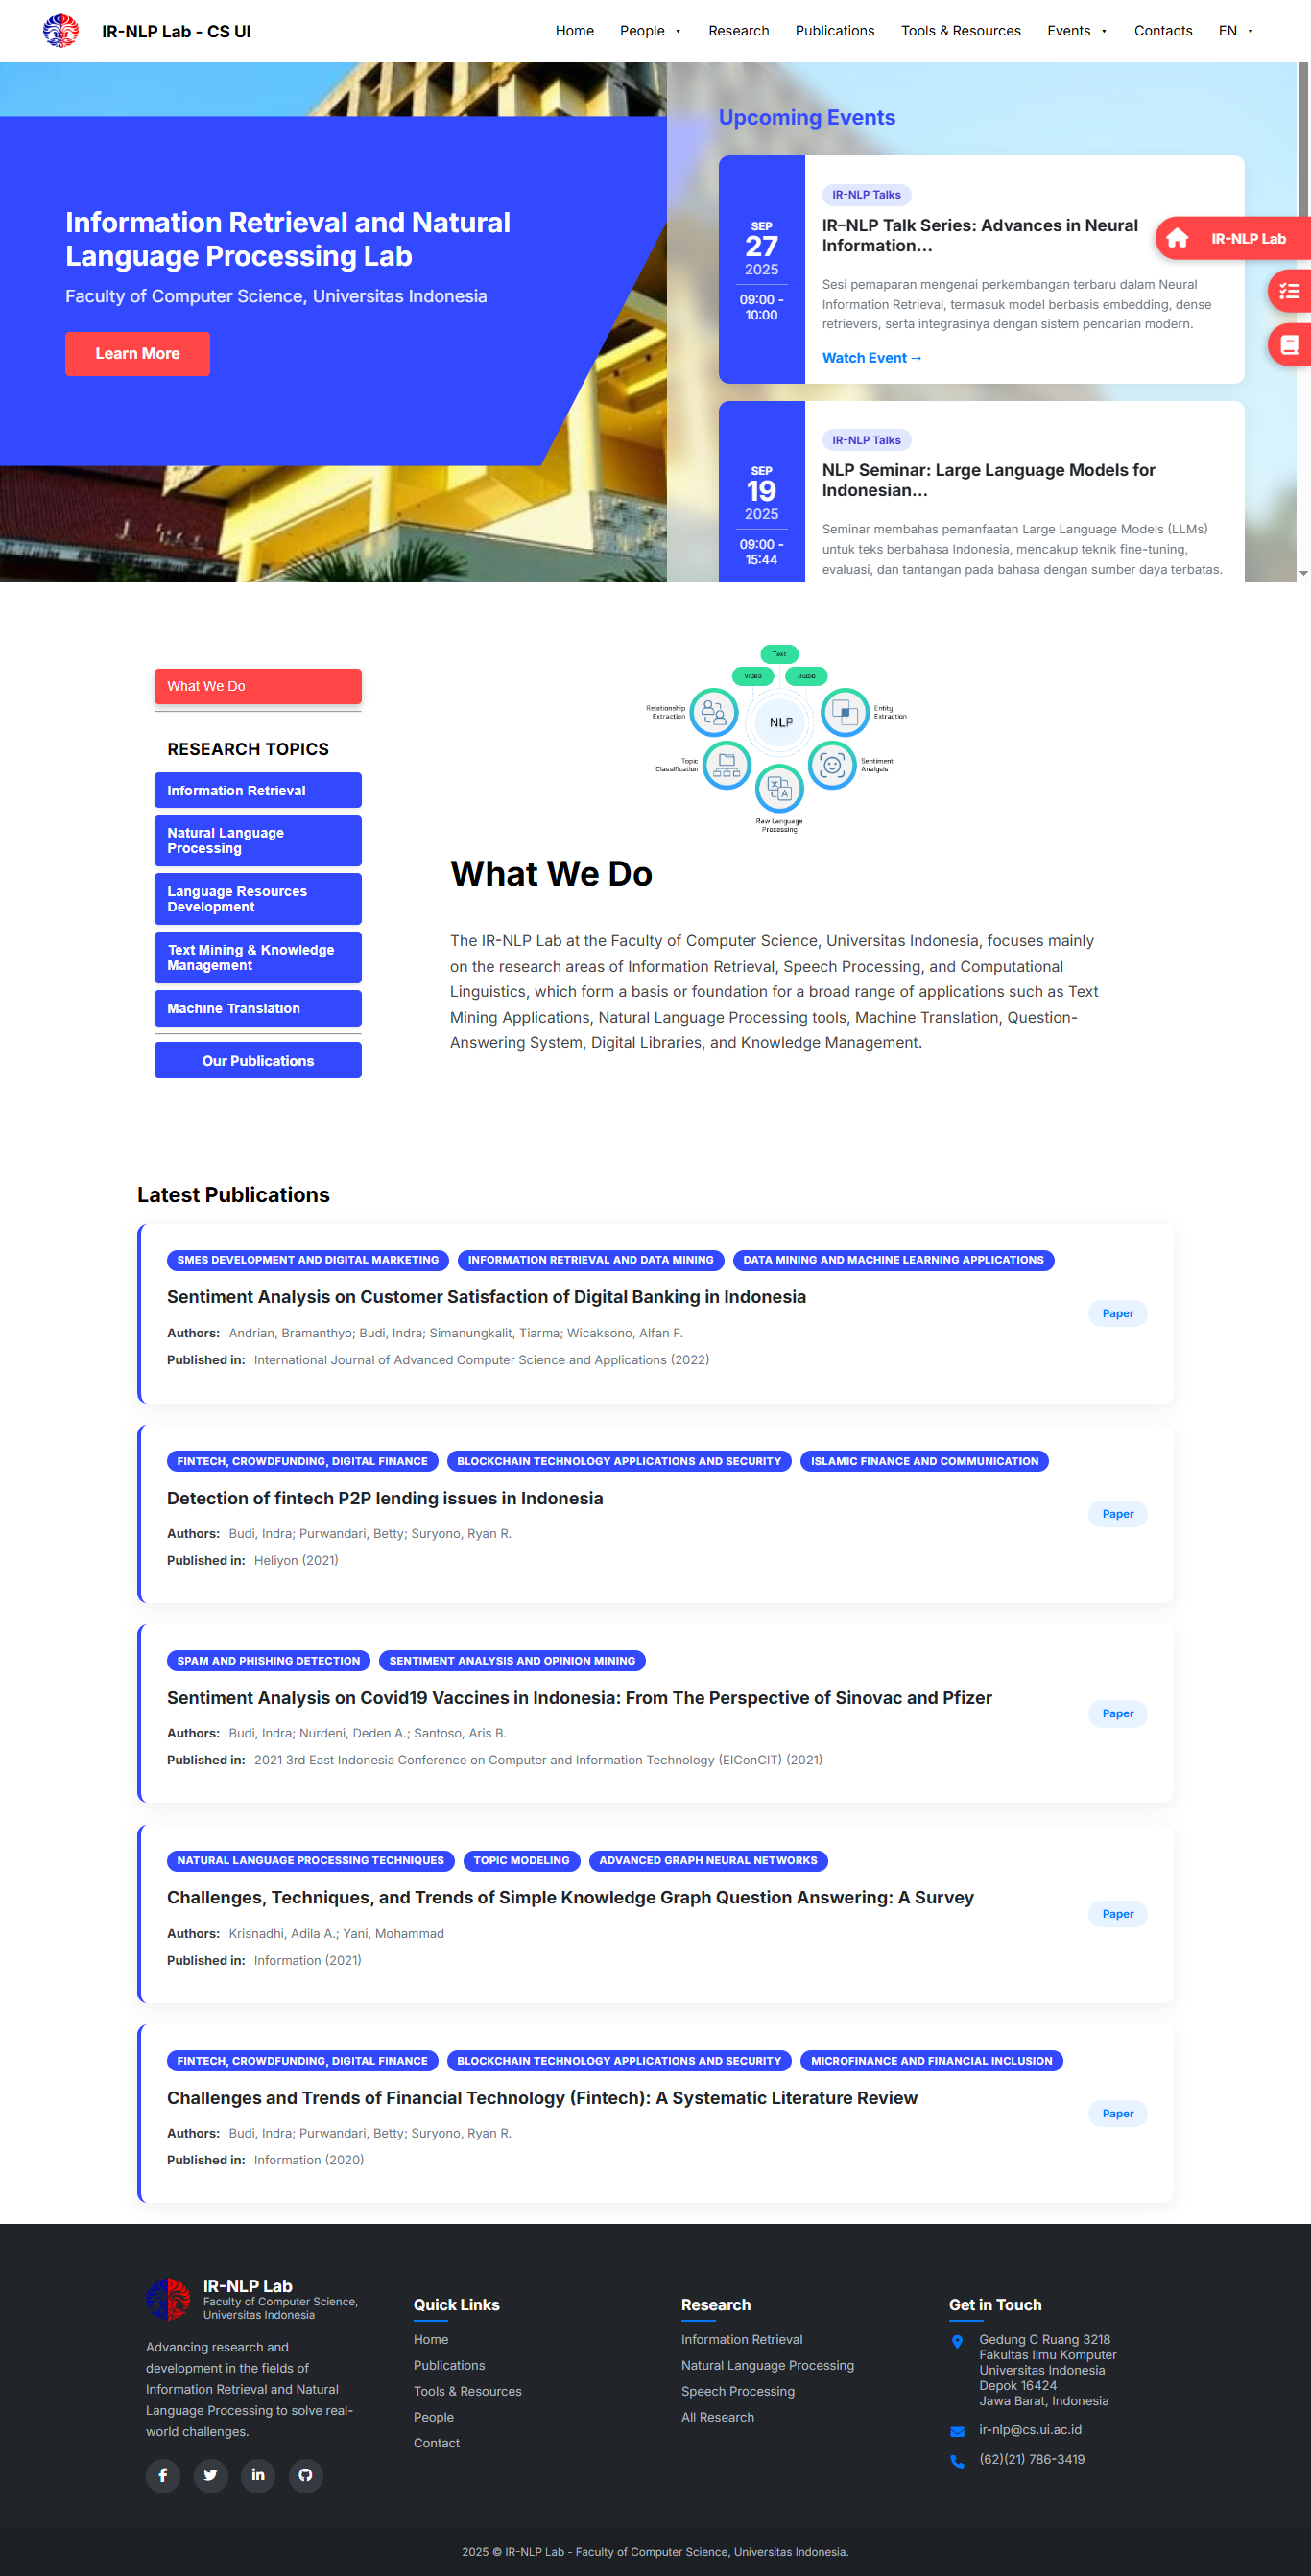
\includegraphics[width=0.7\textwidth]{assets/pics/bab3_homepage.png} 
    \caption{Halaman Homepage}
\end{figure}

\subsubsection{Halaman People}
Menampilkan daftar anggota lab, termasuk dosen, peneliti, mahasiswa, serta peran dan bidang penelitian masing-masing.

\begin{figure}[H]
    \centering
    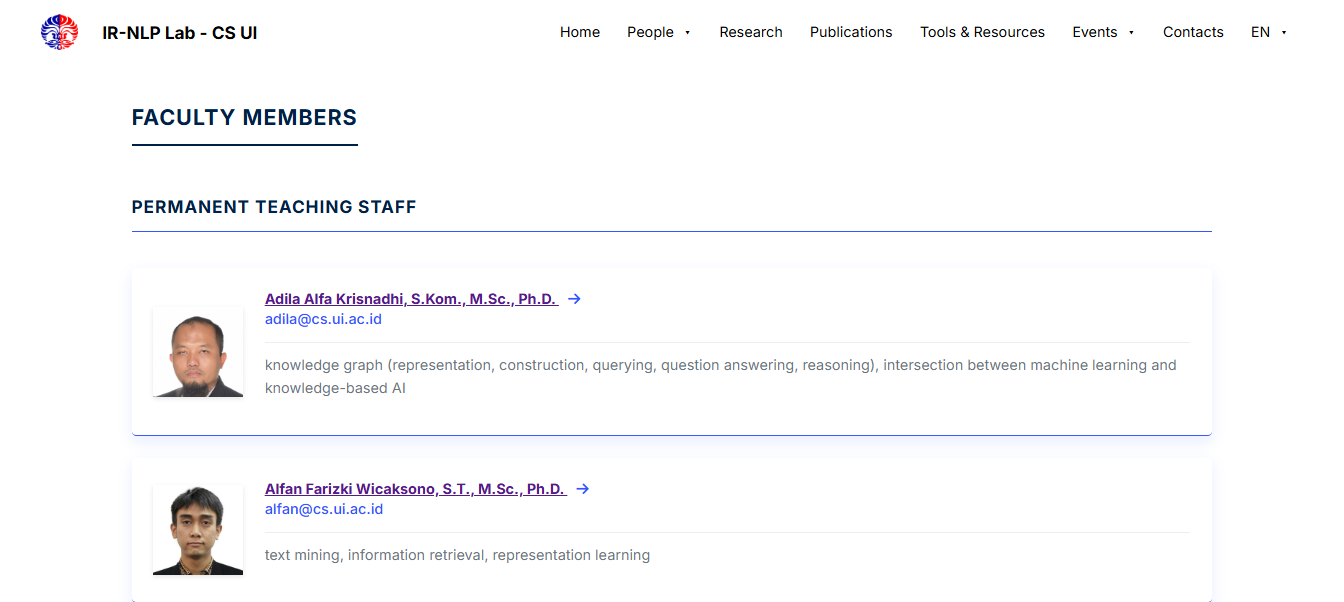
\includegraphics[width=0.7\textwidth]{assets/pics/bab3_faculty_members.png}
    \caption{Halaman People}
\end{figure}

\subsubsection{Halaman Research Grant}
Menampilkan daftar proyek penelitian yang sedang berlangsung maupun yang telah selesai, termasuk sponsor, tahun kegiatan, dan penanggung jawab proyek.

\begin{figure}[H]
    \centering
    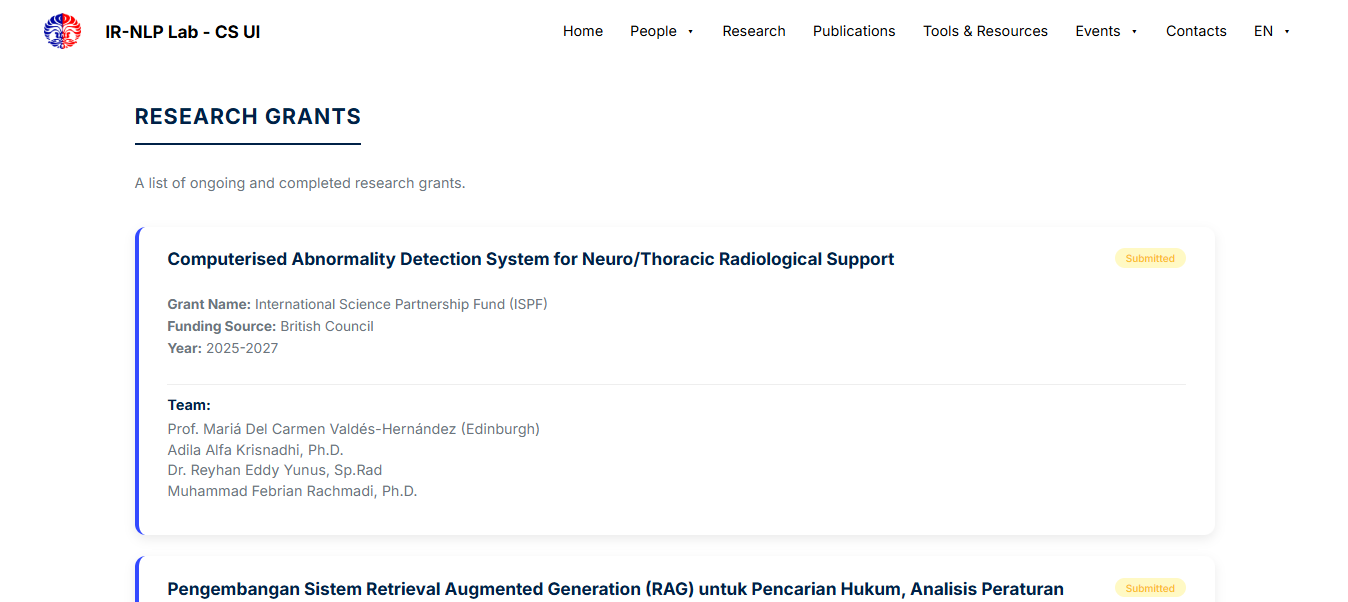
\includegraphics[width=0.7\textwidth]{assets/pics/bab3_research_grants.png}
    \caption{Halaman Research Grant}
\end{figure}

\subsubsection{Halaman Publikasi}
Menampilkan daftar publikasi ilmiah yang diterbitkan oleh anggota lab, seperti jurnal, prosiding konferensi, buku, dan laporan penelitian.

\begin{figure}[H]
    \centering
    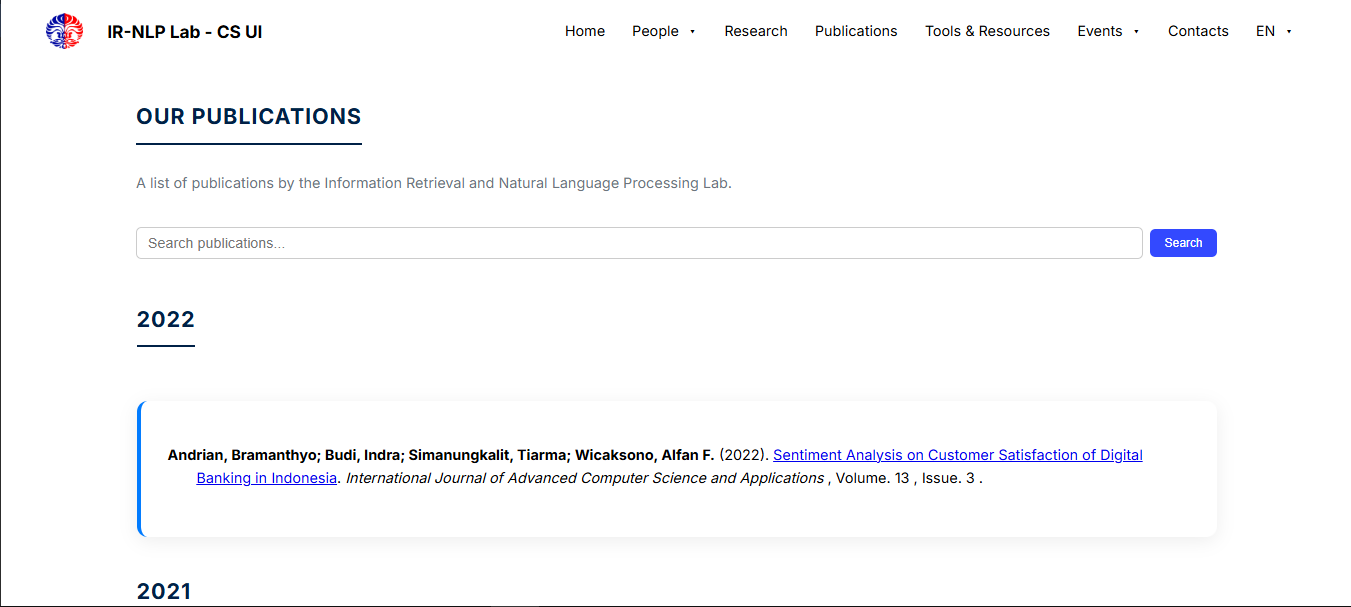
\includegraphics[width=0.7\textwidth]{assets/pics/bab3_publikasi.png}
    \caption{Halaman Publikasi}
\end{figure}

\subsubsection{Halaman Tools and Resources}
Menampilkan beragam tools, dataset, dan perangkat penelitian yang dikembangkan oleh Lab IR-NLP, beserta akses atau dokumentasinya.

\begin{figure}[H]
    \centering
    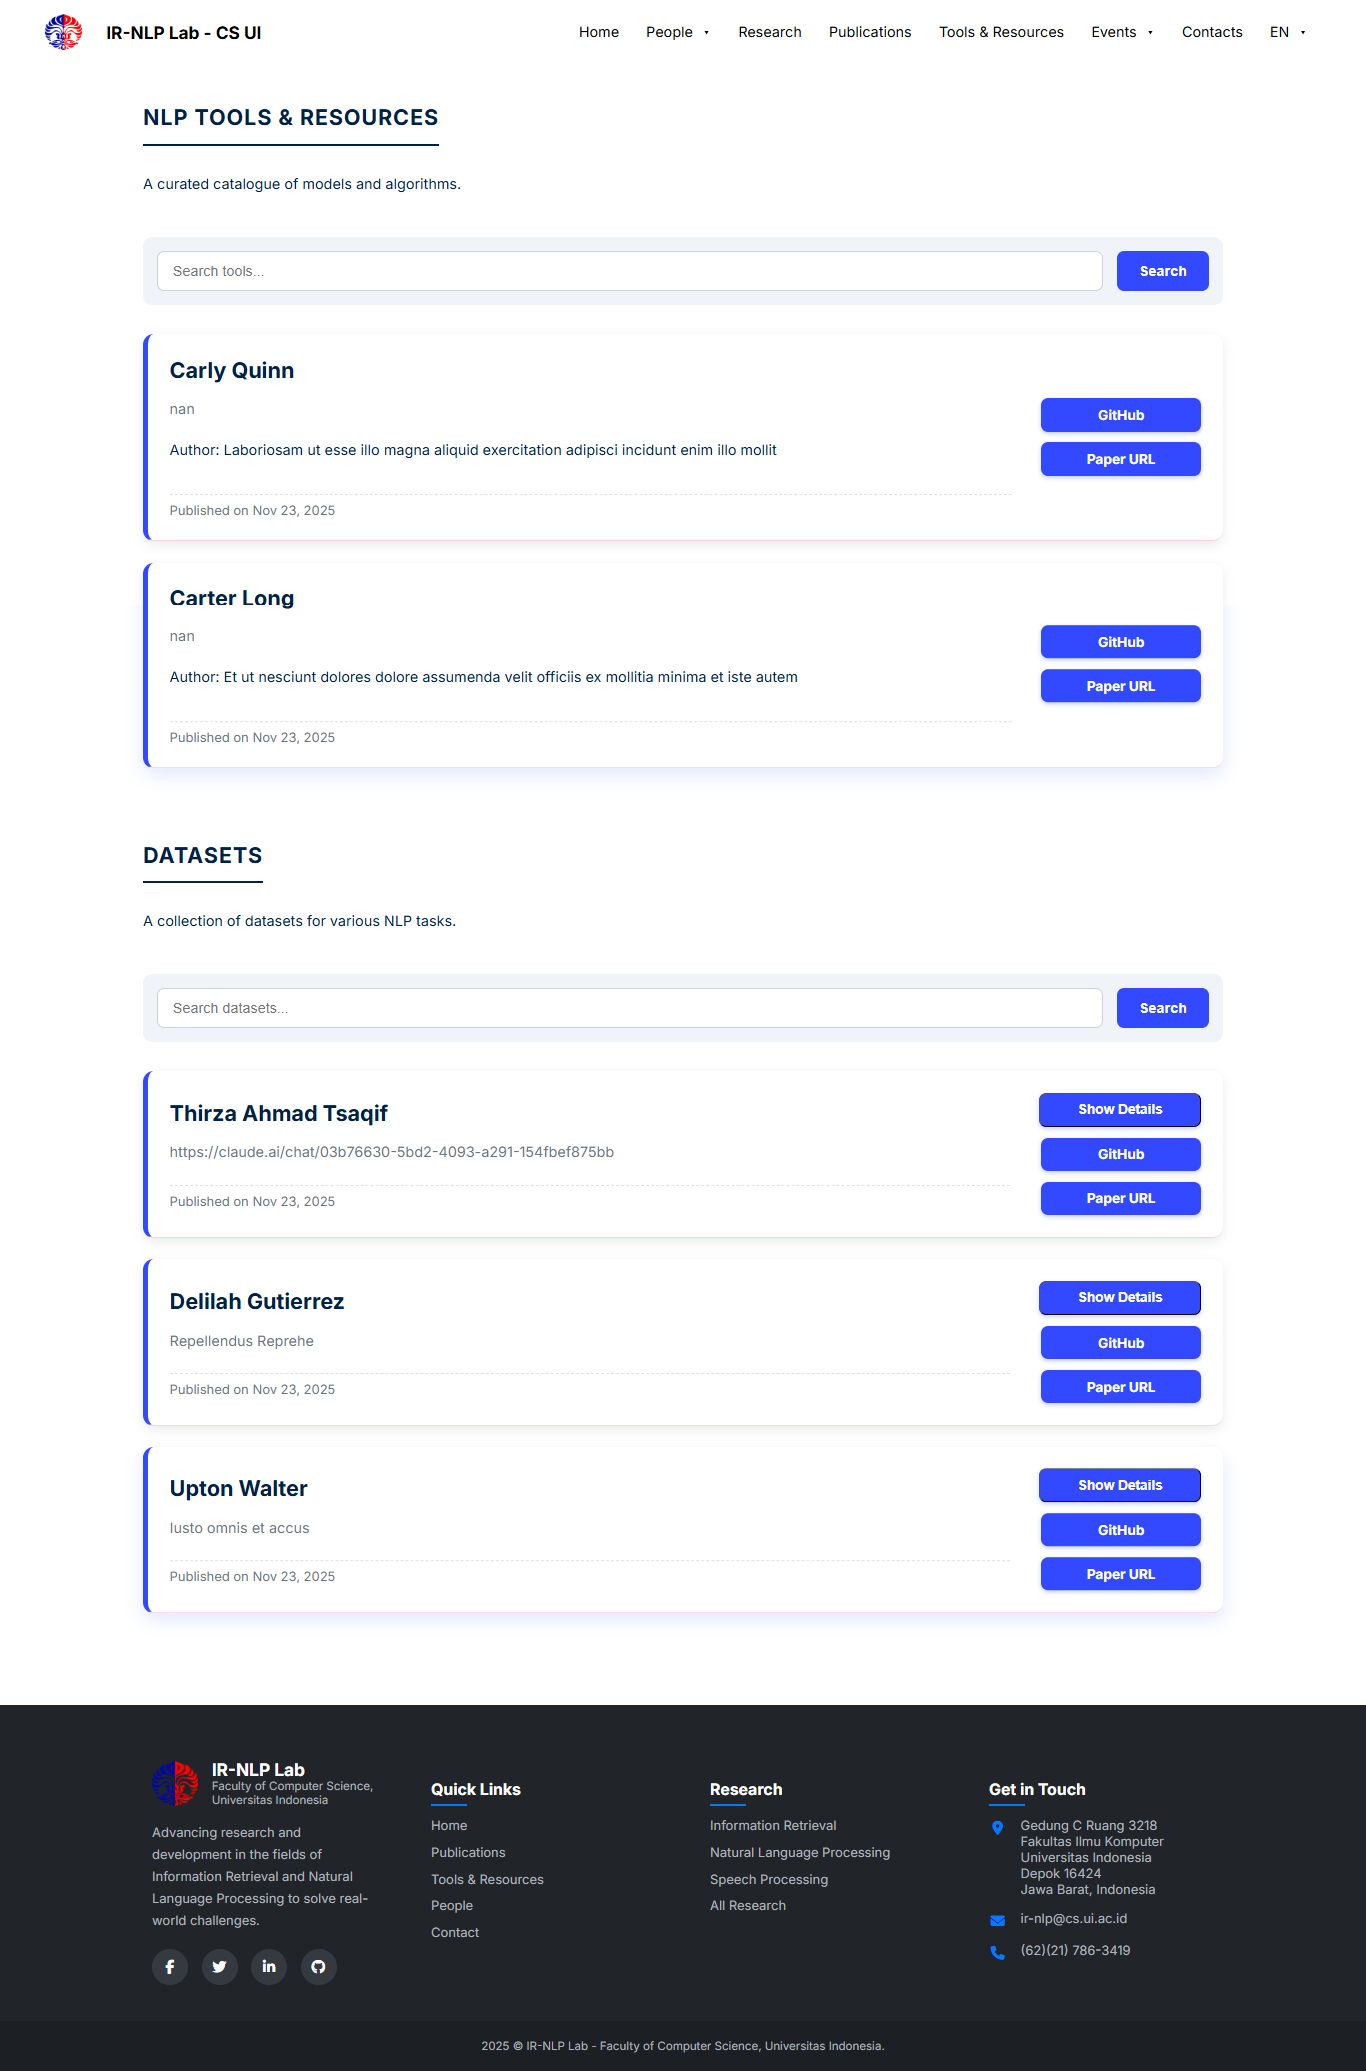
\includegraphics[width=0.7\textwidth]{assets/pics/bab3_tools_and_resources.png}
    \caption{Halaman Tools and Resources}
\end{figure}

\subsubsection{Halaman Events}
Menampilkan daftar acara terkait IR-NLP seperti workshop, seminar, webinar, konferensi, dan kegiatan akademik lainnya.

\begin{figure}[H]
    \centering
    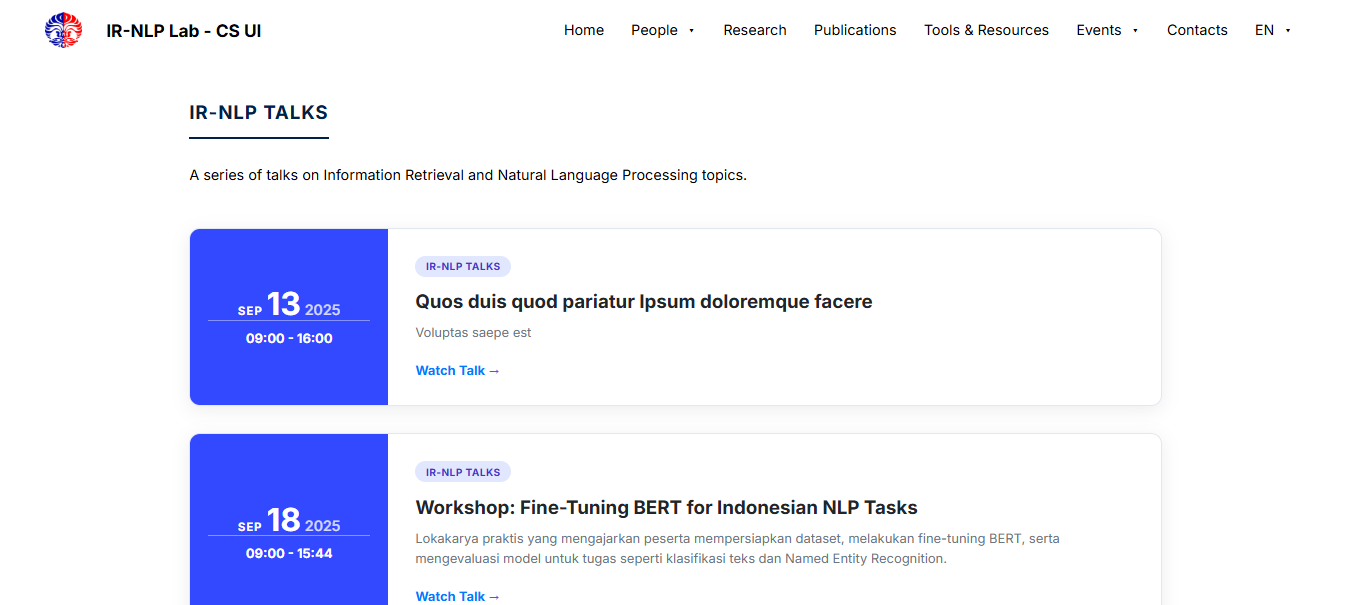
\includegraphics[width=0.7\textwidth]{assets/pics/bab3_events.png}
    \caption{Halaman Events}
\end{figure}

\subsubsection{Halaman Contact}
Menampilkan informasi kontak lab, termasuk alamat, email, dan tautan media sosial untuk menghubungi Lab IR-NLP.

\begin{figure}[H]
    \centering
    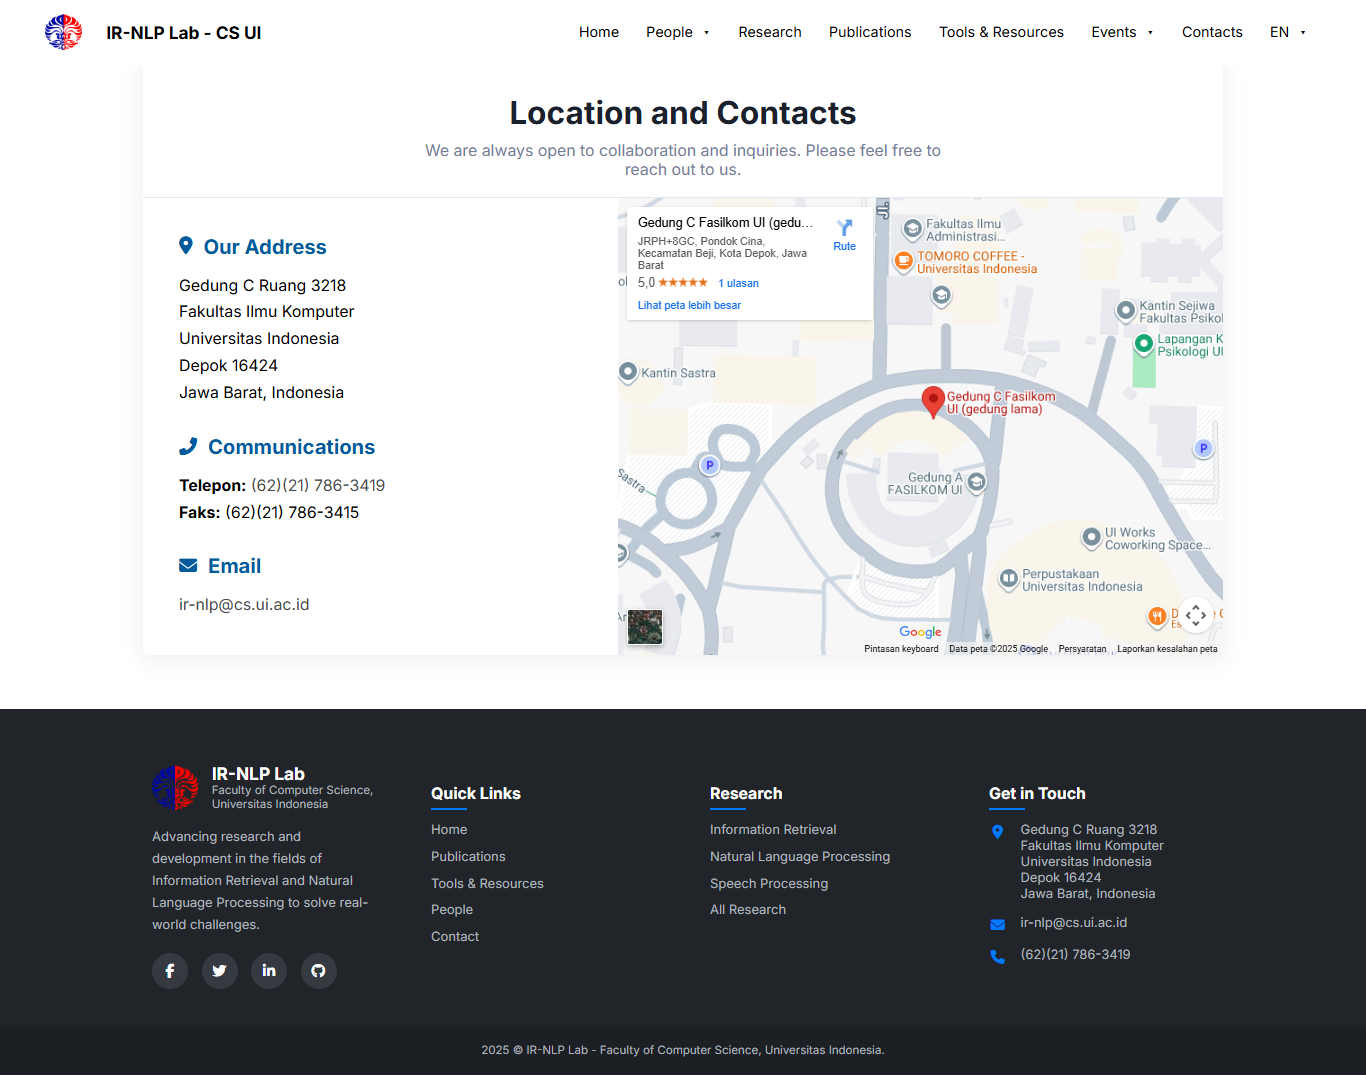
\includegraphics[width=0.7\textwidth]{assets/pics/bab3_contacts.png}
    \caption{Halaman Contact}
\end{figure}

\subsubsection{Halaman Admin}
Halaman ini digunakan untuk melakukan manajemen konten pada website. Melalui halaman admin, pengguna yang memiliki hak akses dapat menambah, mengubah, dan menghapus berbagai elemen konten seperti publikasi hasil \textit{scraping}, anggota lab, acara, \textit{software tool}, dan \textit{dataset}. 

Halaman ini memanfaatkan \textit{Django Admin}, yaitu antarmuka manajemen bawaan dari framework Django yang menyediakan fitur pengelolaan data secara langsung melalui panel administratif. \textit{Django Admin} memungkinkan administrator untuk melakukan operasi \textit{CRUD} dengan cepat, mengatur model yang ditampilkan, serta mengelola hak akses pengguna tanpa memerlukan pembuatan panel admin secara manual.

\begin{figure}[H]
    \centering
    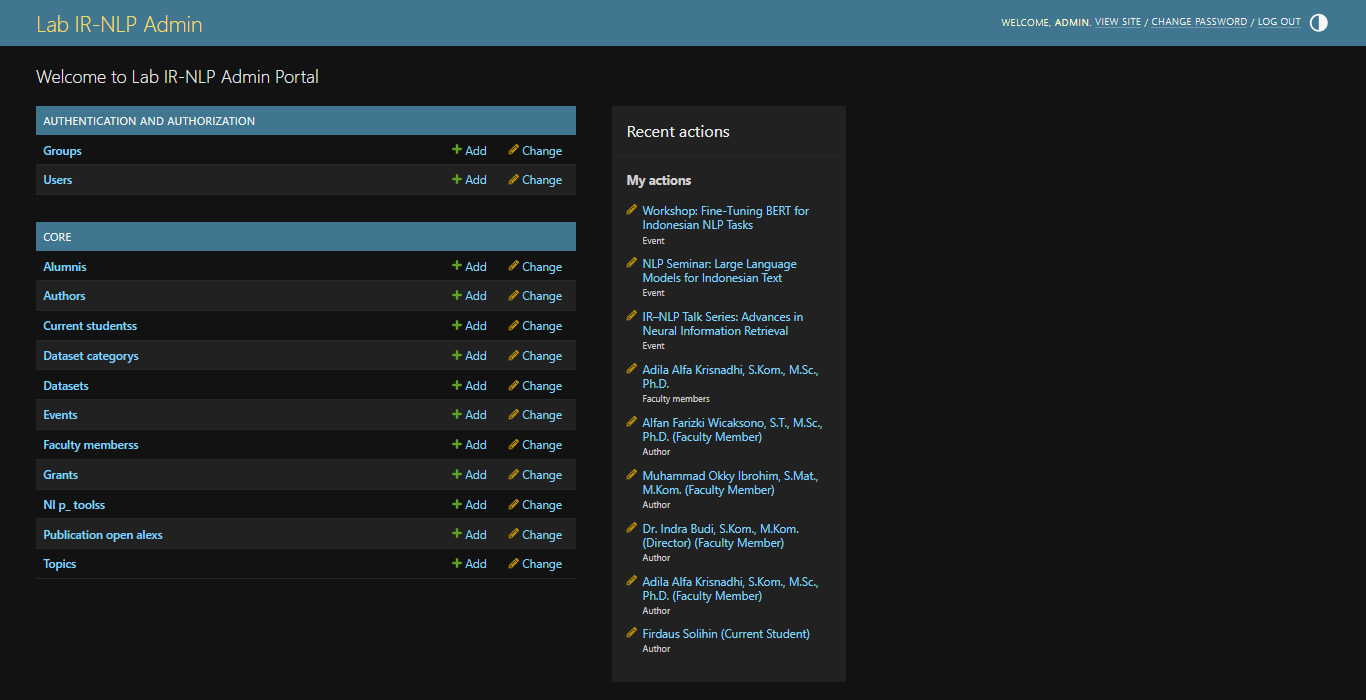
\includegraphics[width=0.7\textwidth]{assets/pics/bab3_admin.png}
    \caption{Halaman Admin}
\end{figure}

\subsection{Metode Pengumpulan Publikasi Berbasis API}
API digunakan sebagai metode utama dalam pengumpulan data karena menyediakan akses langsung, terstruktur, dan terdokumentasi dengan baik terhadap sumber data resmi. Pada sistem ini, API yang digunakan adalah OpenAlex, yaitu layanan indeks terbuka yang menyediakan data publikasi ilmiah, penulis, institusi, topik, dan berbagai metadata terkait. Melalui permintaan (\textit{HTTP request}), sistem memperoleh respons berupa data terformat yang kemudian diproses dan disimpan ke dalam basis data untuk kebutuhan integrasi dan visualisasi pada website.


\begin{figure}[H]
    \centering
    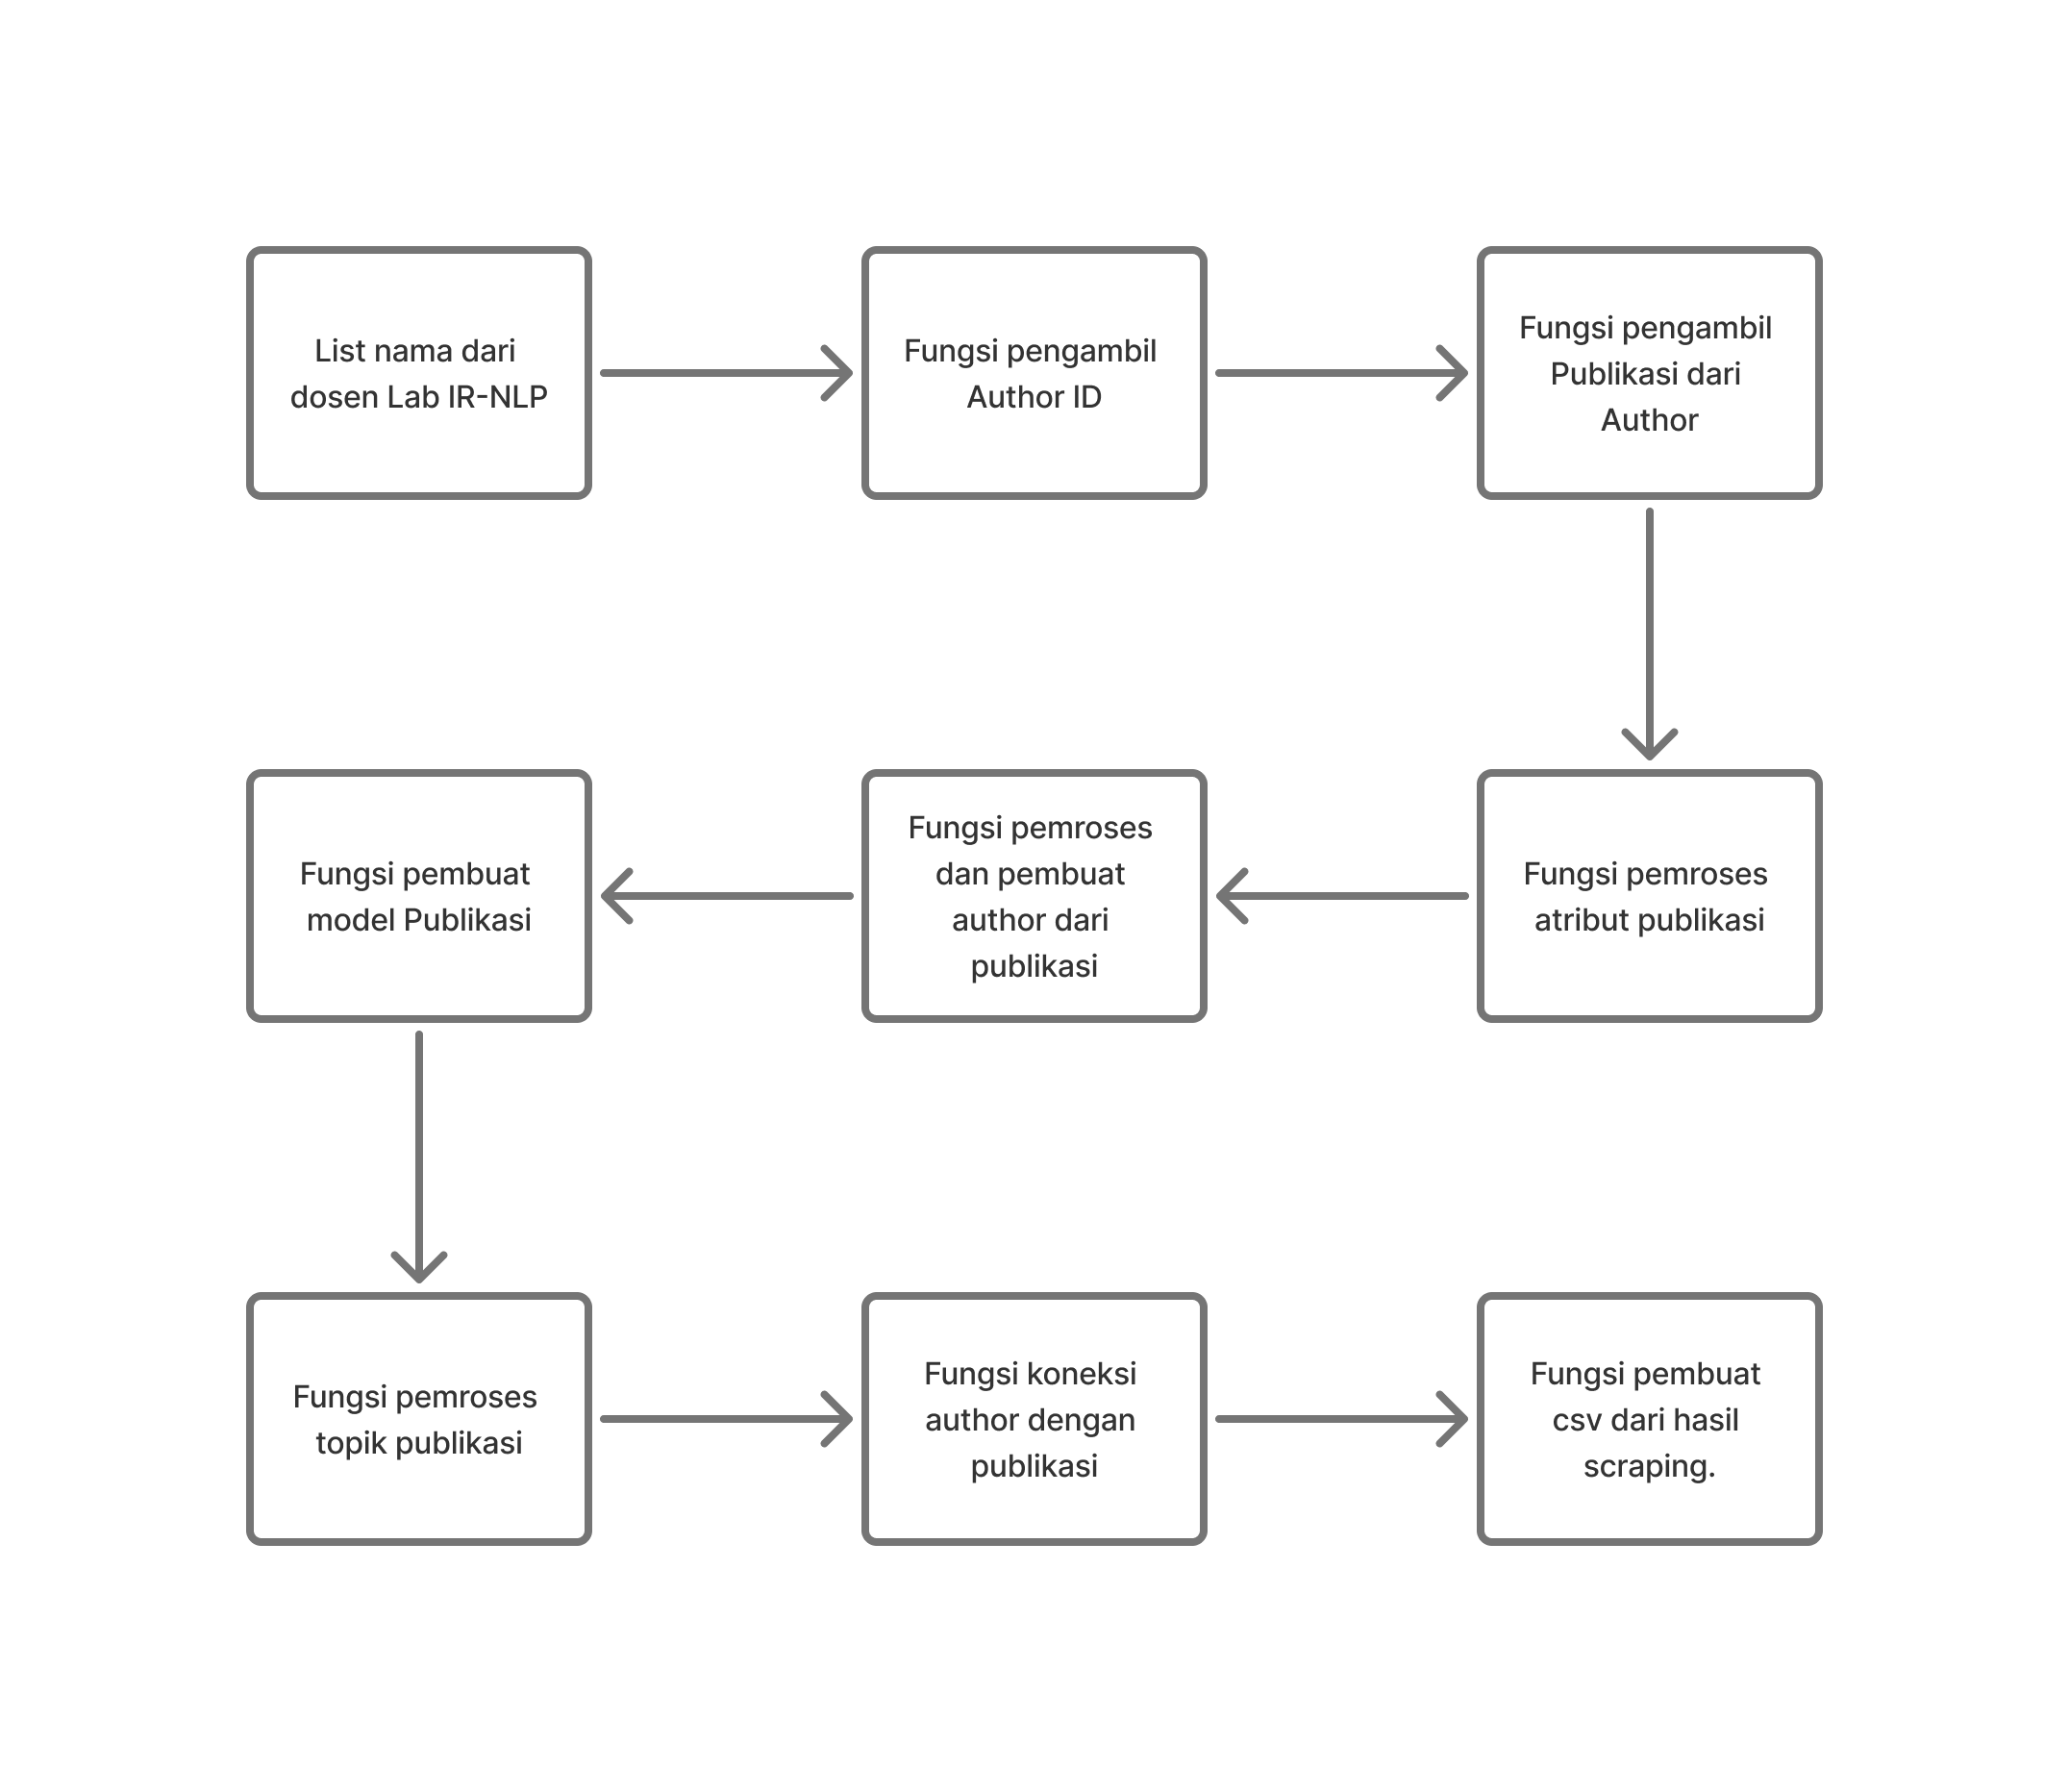
\includegraphics[width=0.7\textwidth]{assets/pics/bab3_api_scraping.png}
    \caption{Alur Pengumpulan Publikasi Menggunakan API}
\end{figure}

Proses pengumpulan publikasi dilakukan dengan langkah-langkah sebagai berikut. Pertama, sistem memiliki daftar nama anggota laboratorium yang publikasinya akan diambil. Daftar tersebut kemudian diiterasi dan masing-masing nama diproses melalui fungsi pencarian \textit{author ID}, karena API OpenAlex hanya menerima dan mengembalikan data publikasi berdasarkan \textit{ID} penulis. Dari tahap ini, sistem memperoleh respons berupa data JSON yang berisi \textit{author ID}.

Selanjutnya, \textit{author ID} tersebut dikirim ke fungsi pengambil publikasi berdasarkan ID penulis. Fungsi ini menghasilkan data JSON yang berisi daftar publikasi lengkap sesuai atribut yang disediakan OpenAlex. Setiap publikasi yang diperoleh kemudian diiterasi dan diproses untuk mengekstraksi atribut yang relevan saja.

Di dalam fungsi pemrosesan publikasi, dilakukan beberapa langkah validasi, seperti:
\begin{enumerate}
    \item pemeriksaan apakah publikasi tersebut sudah pernah disimpan untuk menghindari duplikasi;
    \item pengecekan tipe publikasi untuk memastikan bahwa hanya publikasi berjenis \textit{article} yang diproses.
\end{enumerate}

Tahap berikutnya adalah pemrosesan \textit{authorship}. Pada bagian ini, sistem mengambil informasi mengenai:
\begin{itemize}
    \item \textit{first author},
    \item daftar penulis lain,
    \item judul publikasi,
    \item tahun publikasi,
    \item DOI,
    \item volume dan \textit{issue},
    \item daftar \textit{topics} beserta kategorisasinya,
    \item \textit{primary location} (nama jurnal),
    \item jumlah sitasi,
    \item tanggal publikasi.
\end{itemize}

Atribut \textit{topics} diformat ulang menjadi daftar topik yang dapat disimpan sebagai entitas terpisah. Setelah semua atribut diproses, publikasi disimpan melalui fungsi penyimpanan model publikasi. Setelah publikasi berhasil disimpan ke basis data, dilakukan proses pengaitan relasi menggunakan \textit{foreign key} dan \textit{many-to-many} antara:
\begin{enumerate}
    \item publikasi dan penulis, serta
    \item publikasi dan topik.
\end{enumerate}

Dengan demikian, setiap publikasi yang tersimpan memiliki keterkaitan struktur data yang konsisten, lengkap, dan dapat digunakan untuk kebutuhan tampilan pada halaman publikasi website.


\subsection{Alur Research Grant dari Google Sheets}

Alur pengambilan data \textit{research grant} dimulai dengan melakukan login ke Google Cloud Console, kemudian membuat sebuah proyek baru dengan nama \textit{ir-nlp-grant-scheduler}. Setelah proyek berhasil dibuat, Google Sheets API diaktifkan untuk memungkinkan akses data spreadsheet secara terprogram.

Selanjutnya, dibuat \textit{credentials} berupa \textit{service account} dengan peran (\textit{role}) sebagai \textit{Reader}. Setelah proses pembuatan selesai, dibuat sebuah \textit{key} dalam format JSON yang menghasilkan berkas \texttt{credentials.json}, yang digunakan sebagai kunci autentikasi pada sisi aplikasi.

Tahap berikutnya adalah membuka Google Sheets yang berisi data \textit{grant} IR-NLP, kemudian melakukan proses \textit{sharing} dengan menambahkan alamat email dari \textit{service account} yang telah dibuat sebelumnya, sehingga aplikasi memiliki izin untuk membaca data pada spreadsheet tersebut.

Implementasi teknis dilakukan menggunakan pustaka \textit{google-api-python-client} dan \textit{google-auth} pada bahasa pemrograman Python. Aplikasi mengakses spreadsheet berdasarkan \textit{Spreadsheet ID}, kemudian mendefinisikan lembar kerja (\textit{worksheet}) serta rentang baris yang akan digunakan sebagai sumber data.

Untuk memastikan data selalu terbarui, proses pengambilan data dari Google Sheets dijalankan secara berkala menggunakan \textit{APScheduler}. Dengan pendekatan ini, sistem mampu melakukan pembaruan data secara otomatis tanpa memerlukan intervensi manual.


\subsection{Alur Deployment ke Server Kawung IR-NLP}

Setelah proses pembangunan sistem selesai, tahap selanjutnya adalah melakukan \textit{deployment} aplikasi ke server produksi. Pada penelitian ini, server yang digunakan adalah server Kawung IR-NLP yang dikelola oleh Laboratorium IR-NLP. Proses \textit{deployment} dilakukan secara otomatis menggunakan \textit{GitHub Actions} dengan alur sebagai berikut:

\begin{enumerate}
    \item \textbf{Persiapan Lingkungan Server} \\
    Tahap awal dilakukan dengan memastikan server dapat diakses melalui koneksi \textit{Secure Shell} (SSH) dengan menambahkan \textit{public key} ke dalam berkas \texttt{authorized\_keys}. Selain itu, dilakukan verifikasi spesifikasi perangkat keras dan perangkat lunak server, termasuk memastikan sistem operasi berbasis arsitektur 64-bit dengan menjalankan perintah \texttt{uname -m}, serta memastikan Docker telah terpasang dengan mengecek versi melalui perintah \texttt{docker --version}. Server juga telah dilengkapi dengan lingkungan pendukung seperti Python, Django, dan basis data yang digunakan oleh aplikasi.

    \item \textbf{Konfigurasi Rahasia dan Kredensial} \\
    Seluruh konfigurasi rahasia, seperti \textit{API key}, kredensial basis data, dan variabel lingkungan lainnya, disimpan secara aman menggunakan fitur \textit{GitHub Secrets} pada repositori GitHub untuk menjaga keamanan data sensitif. 

    Khusus untuk berkas \texttt{credentials.json} dari \textit{service account}, berkas tersebut terlebih dahulu dikonversi ke dalam format \textit{Base64} sebelum dimasukkan ke dalam \textit{GitHub Secrets}. Hal ini dilakukan karena \textit{GitHub Secrets} tidak mendukung penyimpanan karakter khusus, seperti tanda petik dua (\texttt{"}), secara langsung. 

    Pada tahap \textit{deployment}, data \textit{Base64} tersebut kemudian didekodekan kembali menjadi berkas \texttt{credentials.json} agar dapat digunakan oleh aplikasi untuk proses autentikasi Google Sheets API.
    \item \textbf{Pembuatan Workflow Deployment} \\
    Dibuat sebuah berkas \texttt{deploy.yaml} pada direktori \texttt{.github/workflows} di dalam repositori GitHub yang berfungsi sebagai konfigurasi otomatisasi \textit{deployment} menggunakan GitHub Actions. Adapun alur kerja pada berkas tersebut adalah sebagai berikut:
    \begin{enumerate}
        \item Workflow dijalankan secara otomatis setiap kali terjadi \textit{push} ke \textit{branch} \texttt{main}.
        \item Pipeline dijalankan pada \textit{runner} berbasis \texttt{ubuntu-latest} dengan \textit{environment} \texttt{production}.
        \item Repository di-\textit{checkout} menggunakan \textit{GitHub Actions}.
        \item Dilakukan autentikasi ke Docker Hub menggunakan \textit{Docker username} dan \textit{Docker password} yang tersimpan pada GitHub Secrets.
        \item Image aplikasi web IR-NLP dibangun (\textit{build}) dan diunggah (\textit{push}) ke Docker Hub sesuai dengan akun pengguna yang telah terautentikasi.
        \item Pada tahap \textit{deployment}, pipeline membuat berkas konfigurasi \texttt{.env} yang berisi variabel lingkungan aplikasi.
        \item Sistem kemudian menginstal dan mengonfigurasi OpenVPN, menghubungkan ke jaringan VPN menggunakan berkas konfigurasi yang tersedia.
        \item Setelah koneksi VPN berhasil, pipeline menyalin berkas konfigurasi \textit{deployment} seperti \texttt{docker-compose.yml}, \texttt{entrypoint}, \texttt{.env}, berkas kredensial \texttt{JSON}, dan konfigurasi \texttt{Nginx}.
        \item Proses dilanjutkan dengan melakukan koneksi SSH ke server Kawung IR-NLP untuk menarik (\textit{pull}) image terbaru dari Docker Hub dan menjalankan aplikasi menggunakan perintah \texttt{docker compose up}.
        \item Setelah aplikasi berhasil dijalankan, koneksi VPN dimatikan untuk mengakhiri proses \textit{deployment}.
    \end{enumerate}

    \item \textbf{Konfigurasi Keamanan SSH} \\
    Untuk menjaga keamanan proses \textit{deployment}, digunakan autentikasi berbasis kunci SSH antara GitHub Actions dan server Kawung IR-NLP sehingga tidak diperlukan penggunaan kata sandi secara langsung.
\end{enumerate}
